\documentclass[tikz,border=4pt]{standalone}
\usepackage{fontspec,amsmath,amssymb,unicode-math}
\setmainfont{STIXTwoText-Regular.otf}[BoldFont=STIXTwoText-Bold.otf,ItalicFont=STIXTwoText-Italic.otf]
\setmathfont{STIXTwoMath-Regular.otf}
\usetikzlibrary{arrows.meta,positioning,calc}
\definecolor{hmtgold}{gray}{0.12}
\definecolor{hmtviolet}{gray}{0.12}
\definecolor{hmtgray}{gray}{0.12}
\definecolor{hmtpaper}{gray}{0.97}
\definecolor{hmtlightgold}{gray}{0.97}
\definecolor{hmtlightviolet}{gray}{0.97}
\begin{document}
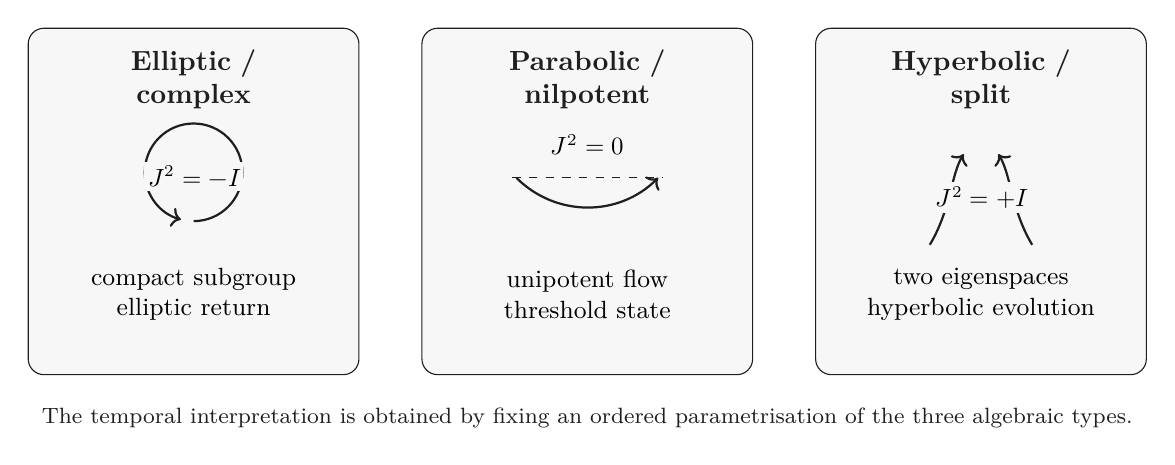
\begin{tikzpicture}[font=\small,box/.style={draw,rounded corners=2mm,minimum width=4.2cm,minimum height=4.4cm,align=center,inner sep=3mm}]
  \node[box,draw=hmtviolet,fill=hmtlightviolet] (ell) at (0,0) {};
  \node[font=\bfseries,align=center,text width=3.6cm,hmtviolet]
    at (0,1.55) {Elliptic /\\complex};
  \draw[hmtviolet,thick,->] (0,-.25) arc (-90:255:.62);
  \node[fill=hmtlightviolet,inner sep=1.5pt] at (0,.32) {\(J^2=-I\)};
  \node[align=center] at (0,-1.18) {compact subgroup\\elliptic return};

  \node[box,draw=hmtgray,fill=hmtpaper] (par) at (5,0) {};
  \node[font=\bfseries,align=center,text width=3.6cm,hmtgray]
    at (5,1.55) {Parabolic /\\nilpotent};
  \draw[hmtgray,thick,->] (4.1,.3) .. controls (4.6,-.2) and (5.4,-.2) .. (5.9,.3);
  \draw[hmtgray,dashed] (4.05,.3)--(5.95,.3);
  \node at (5,.72) {\(J^2=0\)};
  \node[align=center] at (5,-1.18) {unipotent flow\\threshold state};

  \node[box,draw=hmtgold,fill=hmtlightgold] (hyp) at (10,0) {};
  \node[font=\bfseries,align=center,text width=3.6cm,hmtgold]
    at (10,1.55) {Hyperbolic /\\split};
  \draw[hmtgold,thick,->] (9.35,-.55) .. controls (9.62,-.10) and (9.62,.35) .. (9.78,.60);
  \draw[hmtgold,thick,->] (10.65,-.55) .. controls (10.38,-.10) and (10.38,.35) .. (10.22,.60);
  \node[fill=hmtlightgold,inner sep=1.5pt] at (10,.05) {\(J^2=+I\)};
  \node[align=center] at (10,-1.18) {two eigenspaces\\hyperbolic evolution};

  \node[font=\footnotesize,align=center,hmtgray] at (5,-2.75) {The temporal interpretation is obtained by fixing an ordered parametrisation of the three algebraic types.};
\end{tikzpicture}
\end{document}
